\documentclass[aps,prc,preprint,superscriptaddress,showpacs,showkeys]{revtex4-1}
\usepackage{graphicx}
\begin{document}
\title{Cold Nuclear Matter effects in Quarkonia}
These figures shown effect of change in PDF inside nucleus for j/$\psi$ and $\Upsilon$. Calculations have 
flactuations specially as a function of p$_{T}$.

\begin{figure}
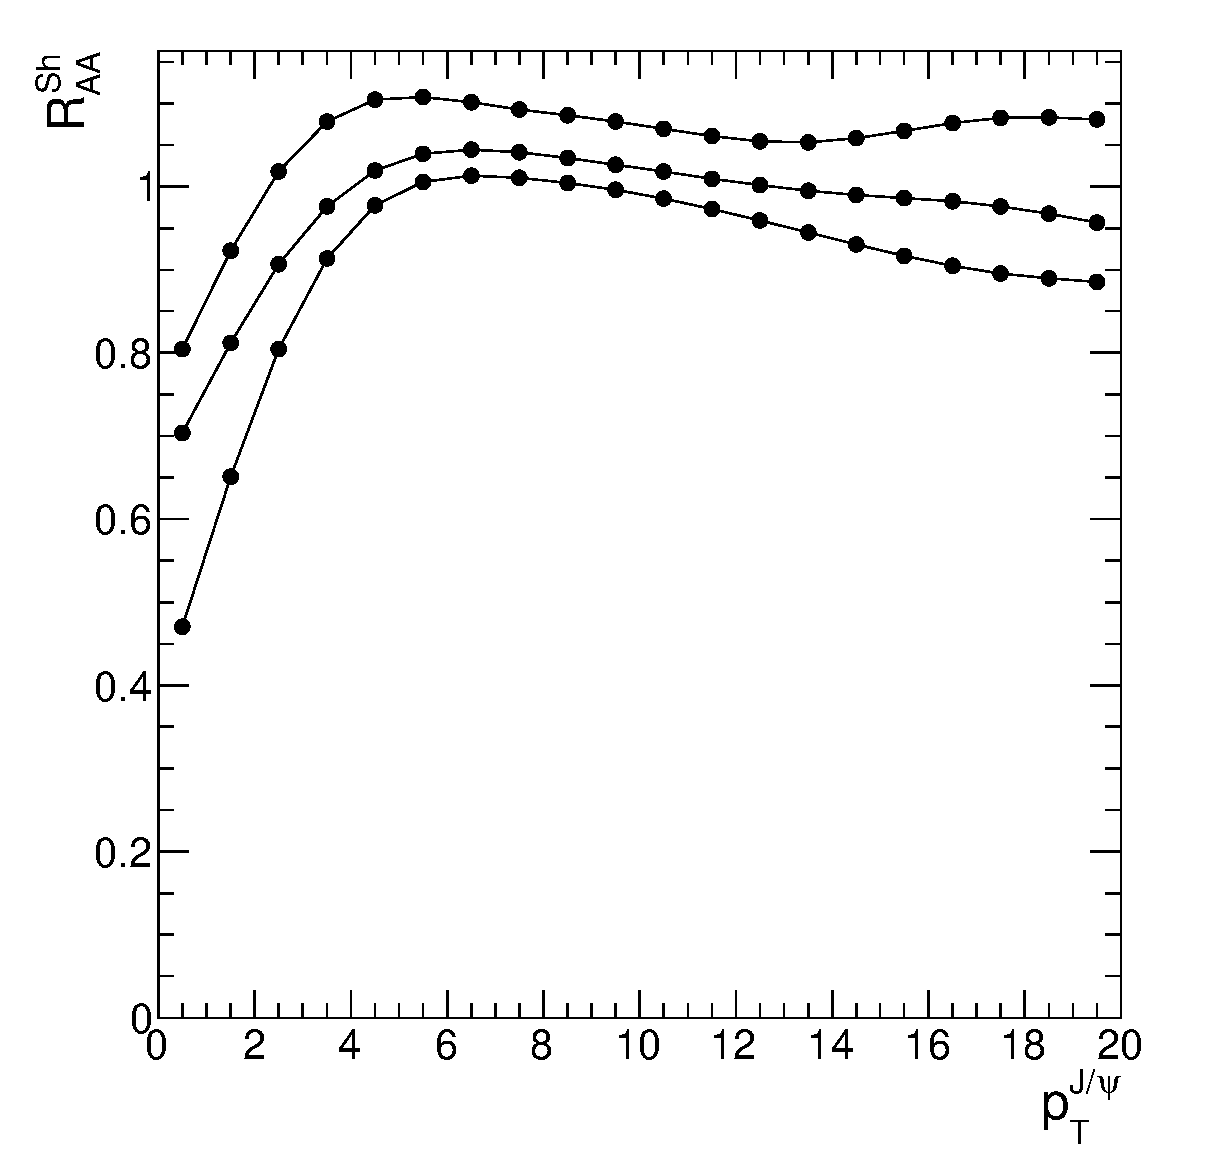
\includegraphics[width=0.49\textwidth]{JpsiRaaShVsPt.eps}
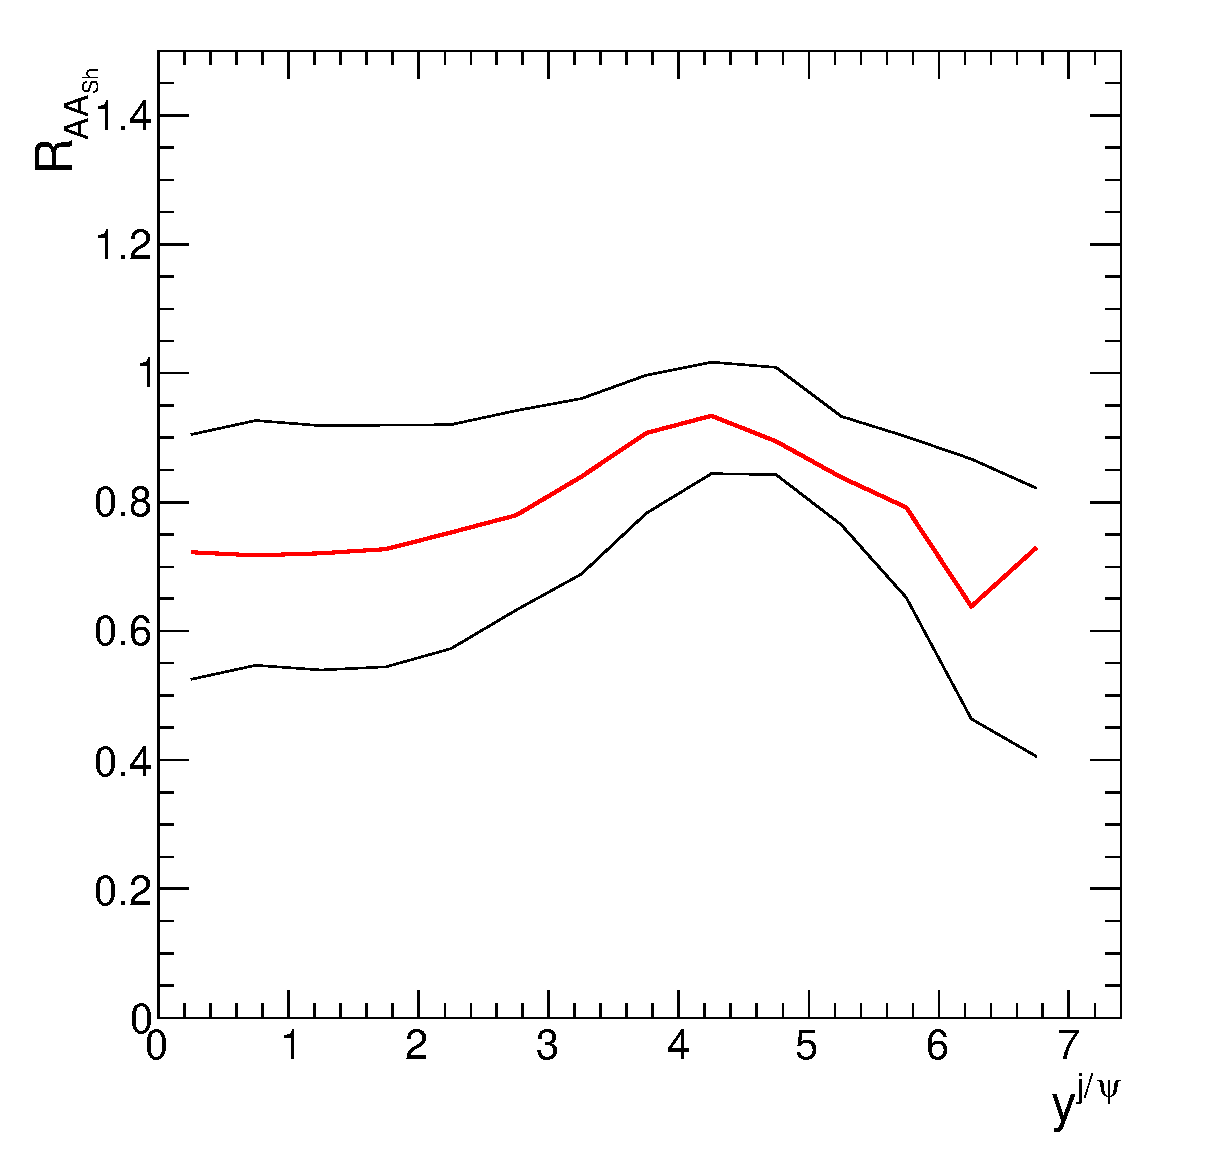
\includegraphics[width=0.49\textwidth]{JpsiRaaShVsRap.eps}
\caption{R$_{AA}$ of j/$\psi$ as a function of p$_{T}$ and rapidity, due to change in parton distribution functions inside nucleus.}
\label{fig:CNMJpsi}
\end{figure}






\begin{figure}
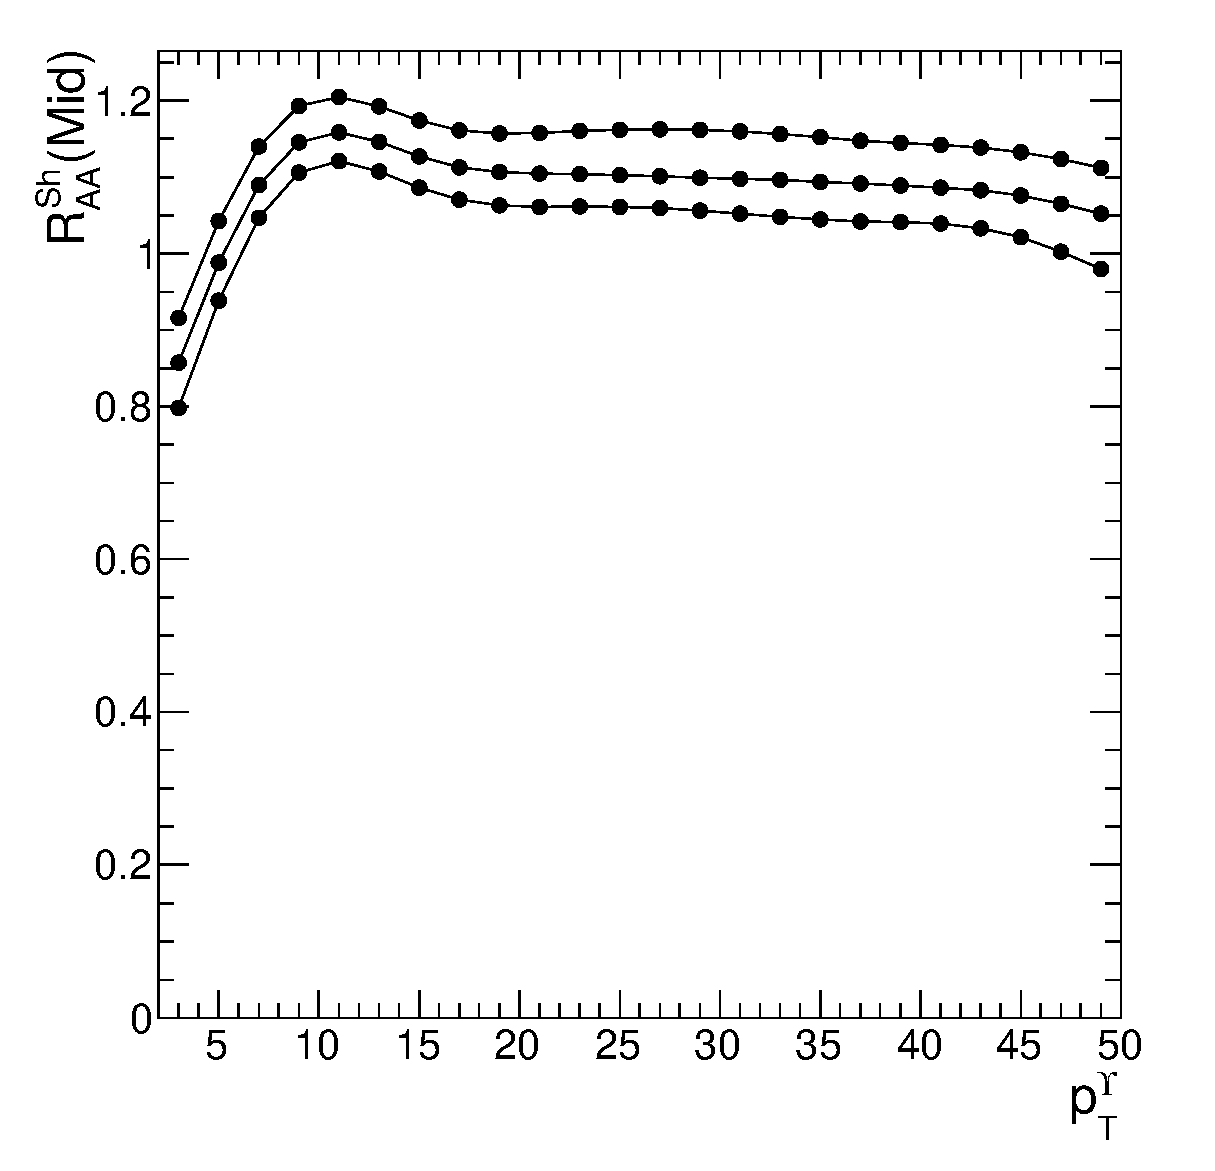
\includegraphics[width=0.49\textwidth]{UpsilonRaaShVsPtMid.eps}
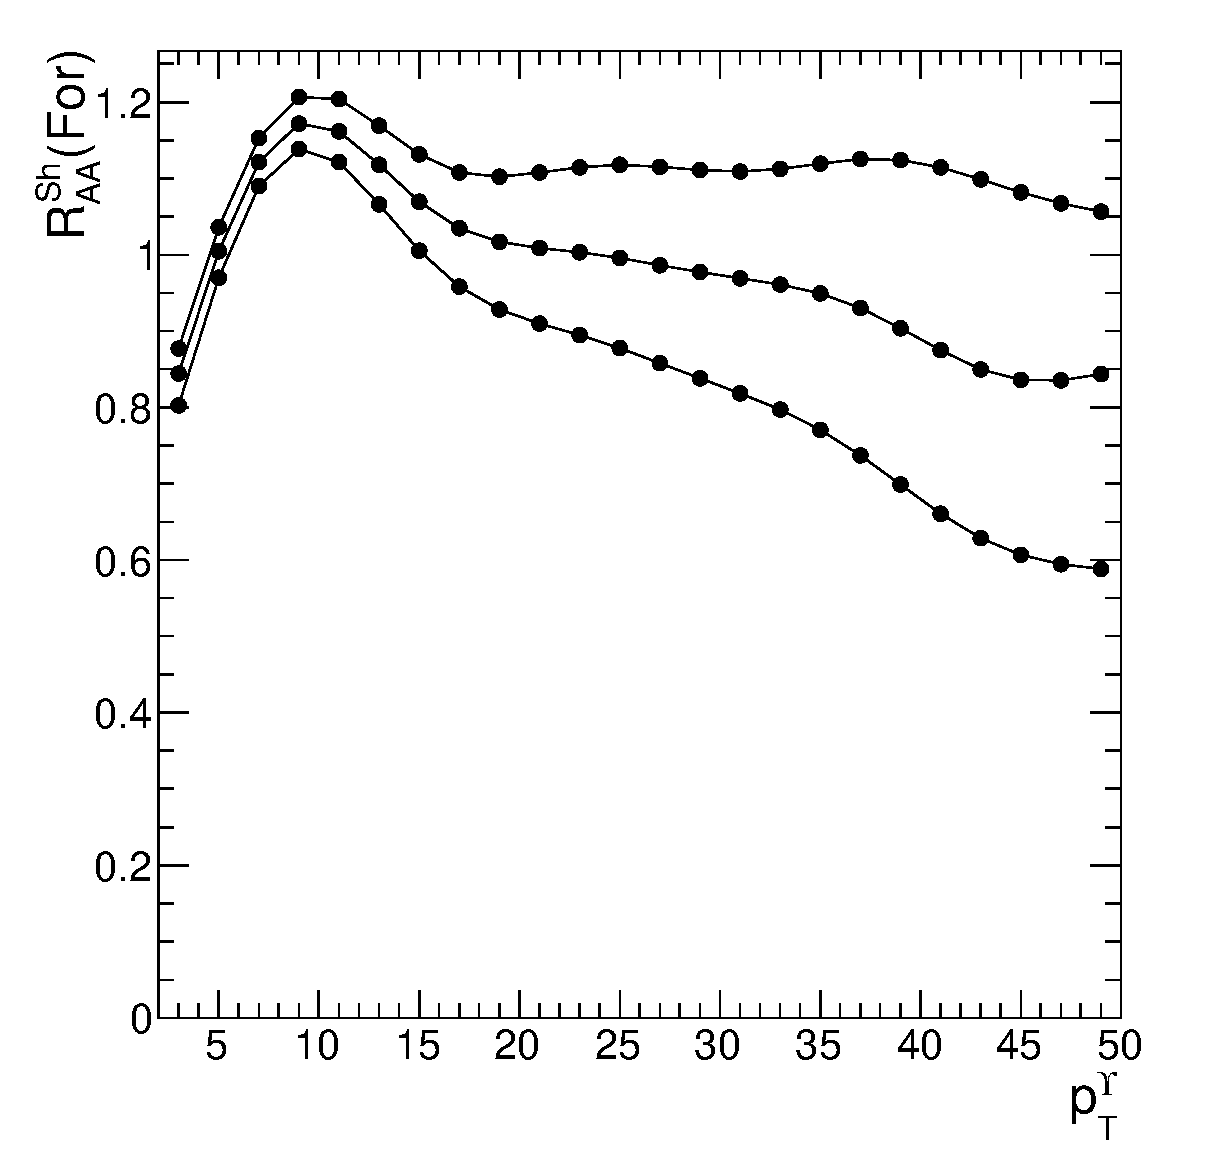
\includegraphics[width=0.49\textwidth]{UpsilonRaaShVsPtFor.eps}
\caption{R$_{AA}$ of $\Upsilon$ as a function of p$_{T}$ in mid(left) and forward(right) rapidity, due to change in parton 
distribution functions inside nucleus.}
\label{fig:CNMUpsilon_Pt}
\end{figure}




\begin{figure}
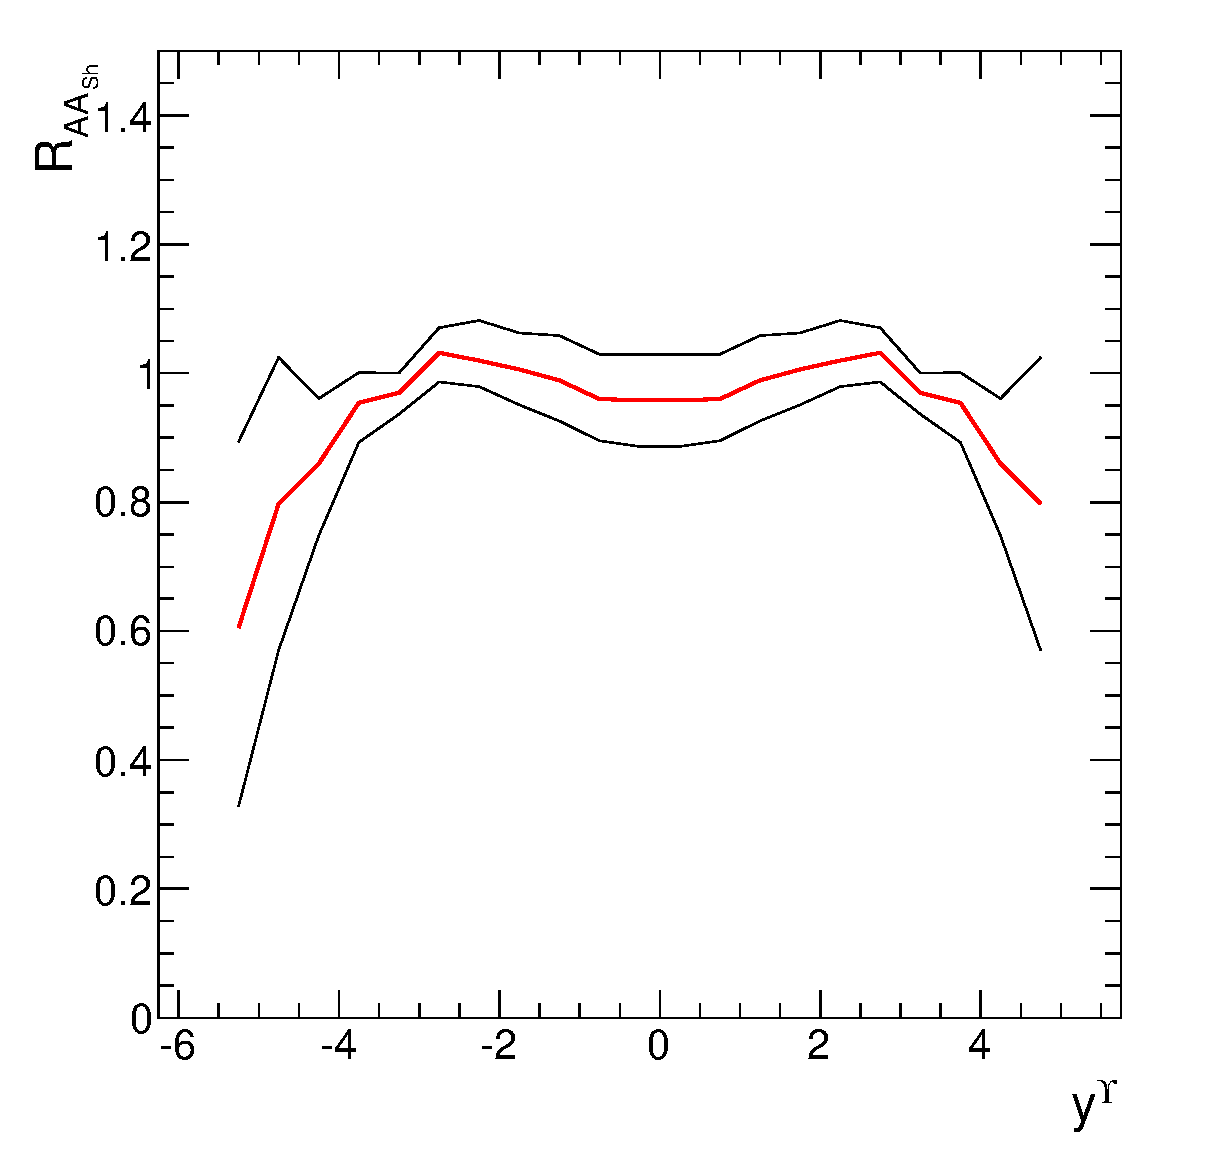
\includegraphics[width=0.49\textwidth]{UpsilonRaaShVsRap.eps}
%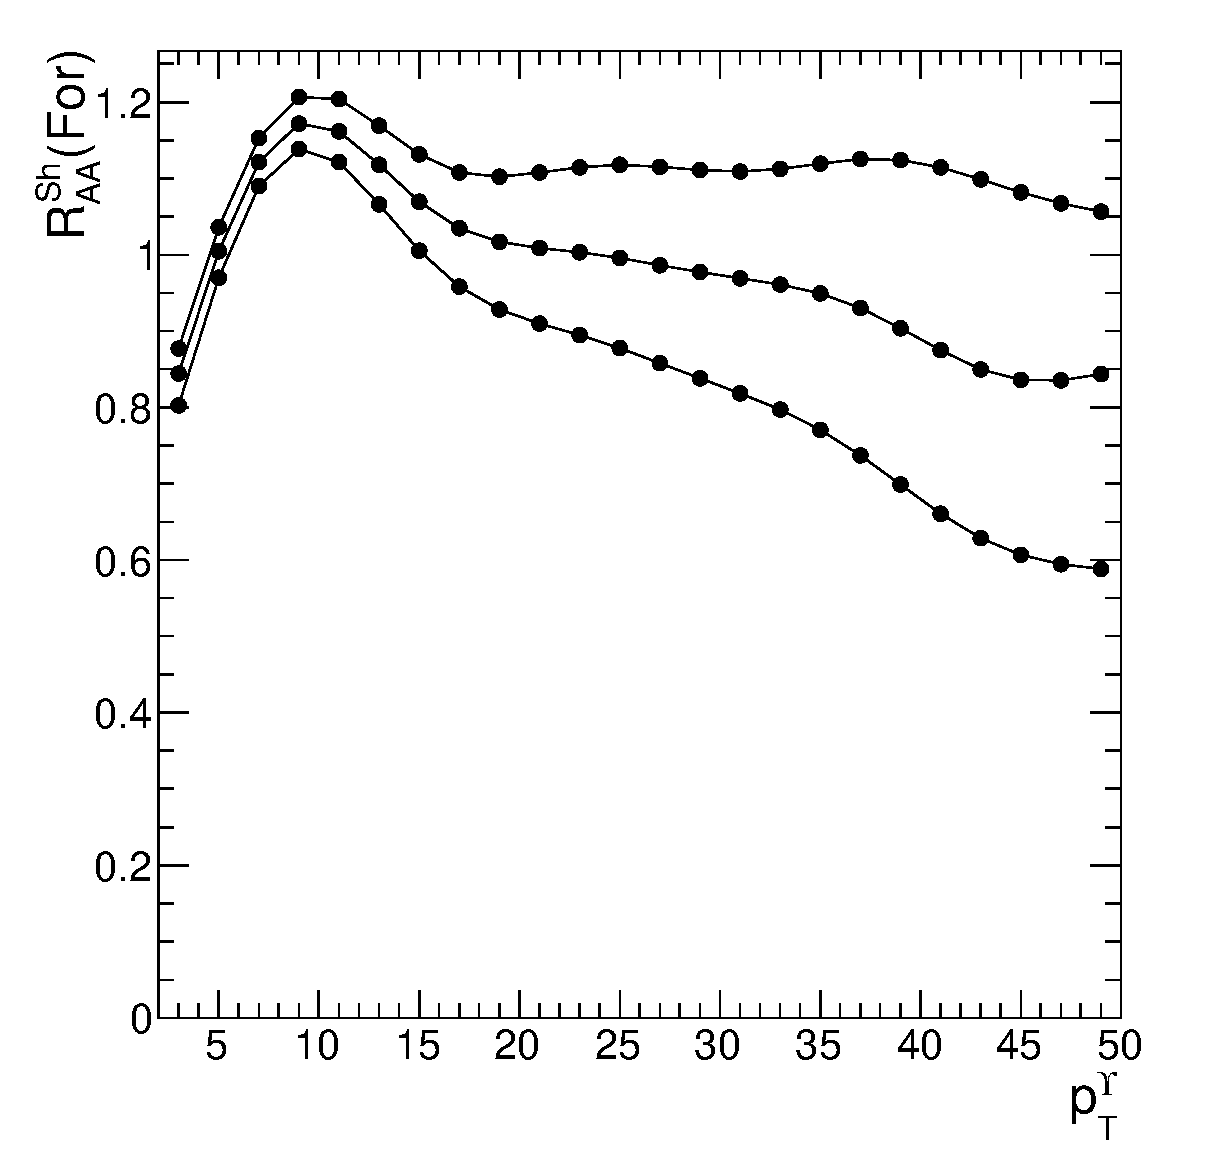
\includegraphics[width=0.49\textwidth]{UpsilonRaaShVsPtFor.eps}
\caption{R$_{AA}$ of $\Upsilon$ as a function of rapidity, due to change in parton 
distribution functions inside nucleus.}
\label{fig:CNMUpsilon_Rap}
\end{figure}






%\begin{figure}
%\includegraphics[width=0.49\textwidth]{}
%\includegraphics[width=0.49\textwidth]{}
%\caption{}
%\label{fig:}
%\end{figure}


\end{document}
